% !TEX root = ../main.tex
%

\section{Results}
\label{sec:results}

\subsection{Main findings}



\begin{enumerate}[nosep, noitemsep]
    \item Unmoderated discussions exhibit significantly worse toxicity and \ac{AQ} (Fig.~\ref{fig::toxicity_aq_stats}) (ANOVA\footnote{The large size and balanced nature of our dataset allows the use of parametric tests.} $p<.000$).

    \item  While the Moderation and Facilitation Guidelines slightly improve \ac{AQ} relative to baselines, their impact is marginal (Fig.~\ref{fig::toxicity_aq_stats}). Notably, these strategies do not reduce toxicity more effectively than the “No Instructions” baseline and perform worse than the “Rules Only” strategy.

    \item Toxicity and \ac{AQ} generally improve over time under all strategies when compared to unmoderated discussions, indicating a limited, but consistent restraining effect caused by the \ac{LLM} moderators over time (Table~\ref{tab:timeseries}).

    \item \ac{LLM} moderators intervene frequently throughout discussions (Fig.~\ref{fig::intervention_count}). \ac{LLM} user-agents exhibit atypical tolerance for excessive moderator interventions, whereas with human participants such repeated interventions often provoke irritation and increased toxicity \cite{schaffner_community_guidelines, make_reddit_great, proactive_moderation, cresci_pesonalized_interventions}.
\end{enumerate}

As expected, our work shows that \ac{LLM} moderators intervening in (synthetic) discussions significantly improves them. Suprisingly however, we fail to find any positive effects of adding sophisticated instruction prompts to \ac{LLM} moderators. This suggests that out-of-the-box \acp{LLM} may not be as adaptable as human moderators. Alternatively, they may lack a high “skill ceiling” which would enable them to effectively use advanced instructions present in current moderation/facilitation manuals. There is also the possibility that our experimental setup constrains the discussions, inhibiting the latent potential of \ac{LLM} moderators, although \ac{LLM} moderators have shown important limitations in discussions with human participants \cite{cho-etal-2024-language}.


\begin{figure*}[t]
    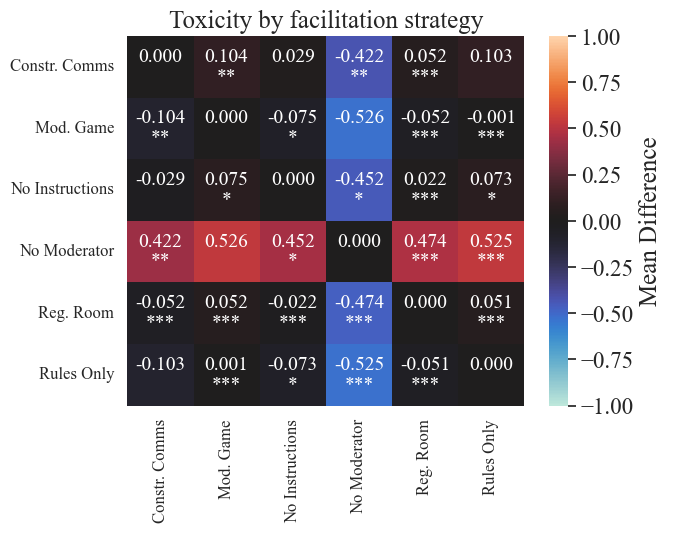
\includegraphics[width=0.49\linewidth]{toxicity_stats.png} \hfill
    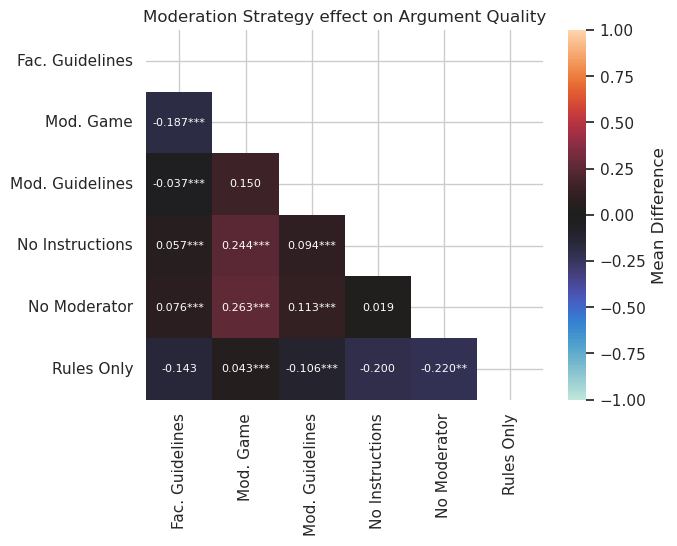
\includegraphics[width=0.49\linewidth]{argumentq_stats.png}
	\centering
	\caption{Mean difference of Toxicity (left) and \ac{AQ} (right) between each moderation strategy. $A[i, j] = 0.3^{***}$ indicates that the strategy $i$ leads to overall worse discussions (more toxicity/worse arguments) compared to $j$ for an average of $0.3$ annotation levels ($1-5$) with $p<.001$. Each comparison is accompanied by pairwise student-t tests, in the form of significance asterisks.}
	\label{fig::toxicity_aq_stats}
\end{figure*}

\begin{figure}
	\centering
	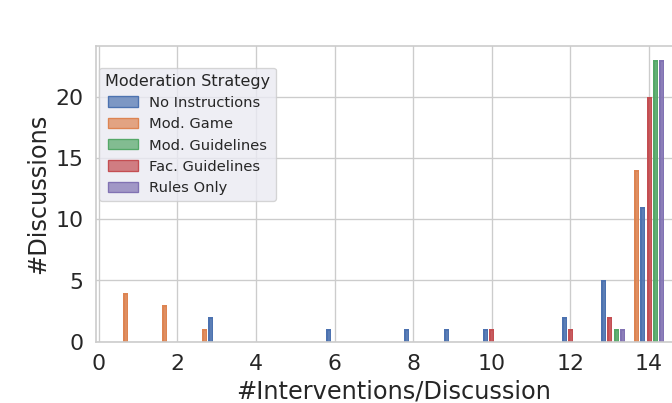
\includegraphics[width=\columnwidth]{intervention_count.png}
	\caption{Histogram of interventions by \ac{LLM} moderators. The maximum number of interventions is $14$.}
	\label{fig::intervention_count}
\end{figure}

\begin{table}
\centering
    \begin{tabular}{lll}
        \toprule
        \textbf{Variable} & \textbf{Toxicity} & \textbf{Arg.Q.} \\
        \midrule
        Intercept & 2.164\textsuperscript{***} & 2.113\textsuperscript{***} \\
        Fac. Guid. & -0.230\textsuperscript{***} & -0.007 \\
        Mod. Guid. & -0.277\textsuperscript{***} & -0.107\textsuperscript{*} \\
        \ac{RL} Game & -0.435\textsuperscript{***} & -0.282\textsuperscript{***} \\
        No Instructions & -0.426\textsuperscript{***} & -0.213\textsuperscript{***} \\
        Rules Only & -0.461\textsuperscript{***} & -0.305\textsuperscript{***} \\
        time & -0.012\textsuperscript{**} & -0.012\textsuperscript{**} \\
        Fac. Guid$\times$time & -0.023\textsuperscript{***} & -0.024\textsuperscript{***} \\
        Mod. Guid$\times$time & -0.023\textsuperscript{***} & -0.011\textsuperscript{*} \\
        \ac{RL} Game$\times$time & -0.011\textsuperscript{*} & 0.003 \\
        No Instructions$\times$time & -0.003 & 0.003 \\
        Rules Only$\times$time & -0.008 & -0.002 \\
        \bottomrule
    \end{tabular}
    \small
    $\cdot p<0.1$, \textsuperscript{*} $p<0.05$, \textsuperscript{**} $p<0.01$, \textsuperscript{***} $p<0.001$
    \normalsize
    \caption{OLS Regression Coefficients for Toxicity ($Adj. R^2=0.054$) and \ac{AQ} ($Adj. R^2=0.016$). \textit{“Time”} denotes dialogue turn, reference factor is \textit{“No moderator”}.}
    \label{tab:timeseries}
\end{table}



\subsection{Ablation study}
\label{ssec:results:ablation}

We test the effects of our proposed methodology by running $8$ synthetic discussions using the Qwen 2.5 model, and comparing their \textit{diversity} scores (Section \ref{ssec:methodology:diversity}) with our original dataset, as well as with human discussions. We use the Cornell eRulemaking “Regulation Room” dataset \footnote{\url{http://archive.regulationroom.org} Any opinions, findings, and conclusions or recommendations expressed in this material are those of the author(s) and do not necessarily reflect the views of the \ac{CeRI}}, from which we extract all comments from all initiatives. 


\subsubsection{Quality of model outputs}

Among the evaluated models, Qwen exhibited the highest diversity, suggesting limited participant interaction (Section~\ref{ssec:methodology:diversity}), followed by Mistral Nemo and LLaMa (Fig.~\ref{fig::diversity}). None of the models closely approximated human discussions in terms of diversity, although Mistral achieved the most human-like comment length (Fig.~\ref{fig::comment_length}). Notably, LLaMa's low diversity may be caused by its longer comment lengths, as evidenced by a statistically significant negative correlation between comment length and diversity in synthetic discussions ($p<.000$), which is absent in human texts ($p=0.775$). These findings align with prior work \cite{Park2023GenerativeAI, leng_2024} that suggests that intensly aligned \acp{LLM} like LLaMa struggle to mimic authentic conversational dynamics. Nevertheless, the difference in their performance is small enough that we can not endorse any single model for accurate simulation of real-world discourse.


\subsubsection{Effects of turn taking algorithms}

We assess three methods for controlling user turns: Round Robin (placing each participant in a predetermined queue), Random Selection, and our own approach (Section~\ref{ssec:experimental:turn}). Although no single function fully replicates human diversity (Fig.~\ref{fig::diversity}), both traditional methods yield discussions with extremely high diversity scores, deviating significantly from human norms. Our proposed algorithm improves synthetic conversations by reducing this divergence, demonstrating meaningful positive effects on data quality that cannot be attributed to comment length alone (Fig.~\ref{fig::comment_length}).


\subsubsection{Effects of user-agent prompting}

We run discussions where user-agents (1) are not assigned \acp{SDB}, (2) are not assigned roles, and (3) are given a basic instruction prompt (see Appendix~\ref{sssec:appendix:actors}). Fig.~\ref{fig::diversity} demonstrates that, while our approach (using roles, \acp{SDB}, and our improved instruction prompt) is not enough to create synthetic discussions with similar diversity as human discussions, removing any of its aspects leads to a significant divergence. This divergence is similar to the one observed when changing the turn taking function, and can similarly not be attributed to differences in comment length (Fig.~\ref{fig::comment_length}).

Interactions involving “Troll” user-agents, directed by our finetuned instruction prompt, led to increased toxicity and decreased \ac{AQ} among other participants (Student's t-test, $p < .000$), even when moderated under the “No Instructions” strategy. This effect diminishes when explicit instructions to react to toxic posts are removed (Fig.~\ref{fig::boxplots}), with a similar, though less pronounced, impact on \ac{AQ}. These findings suggest that finetuned instruction prompts are essential for eliciting behaviors which moderators can take action against.

\begin{figure*}[t]
    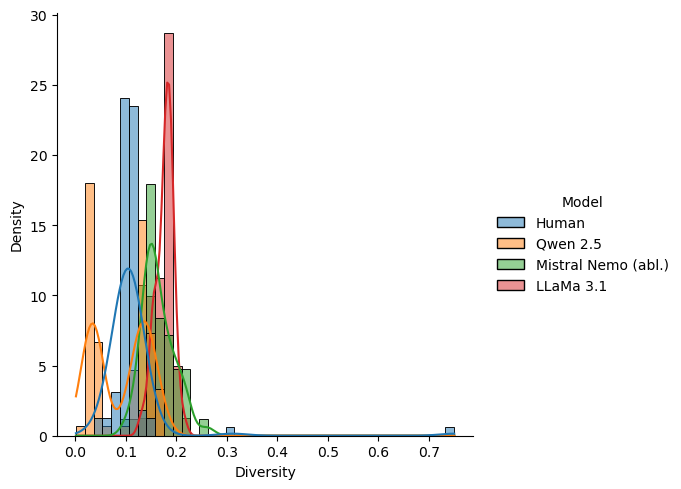
\includegraphics[width=0.32\linewidth]{rougel_model.png} \hfill
    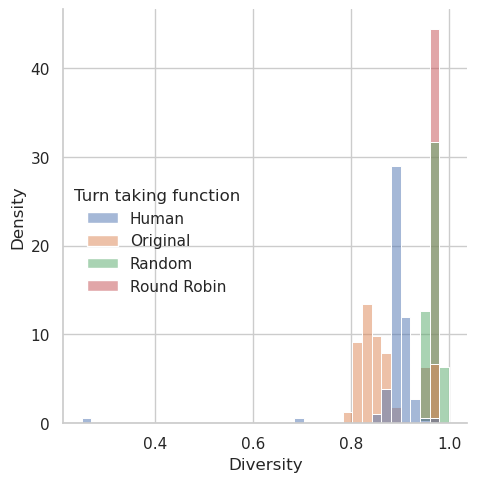
\includegraphics[width=0.32\linewidth]{rougel_turns.png}
    \hfill
    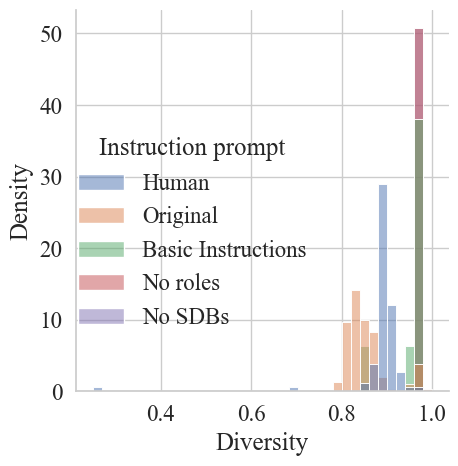
\includegraphics[width=0.32\linewidth]{rougel_prompts.png}
	\centering
	\caption{Diversity (Section~\ref{ssec:methodology:diversity}) distribution for each discussion by model (Section~\ref{ssec:experimental:model}), turn-taking function $u$ (Section~\ref{ssec:experimental:turn}), and prompting function $\phi$ used (Section~\ref{ssec:experimental:prompts}).}
	\label{fig::diversity}
\end{figure*}

\begin{figure*}[t]
    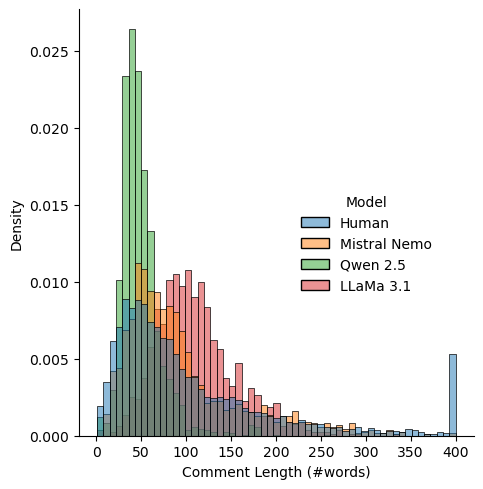
\includegraphics[width=0.32\linewidth]{comment_len_model.png} \hfill
    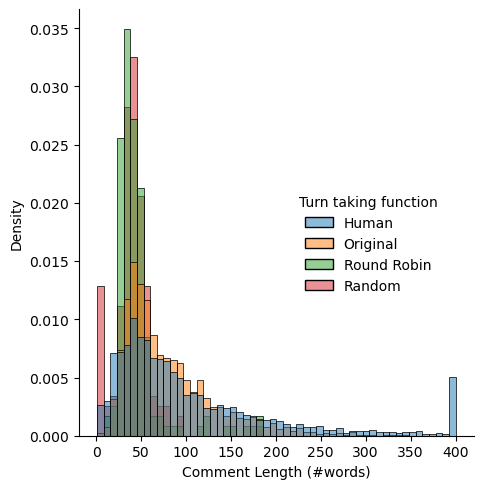
\includegraphics[width=0.32\linewidth]{comment_len_turns.png}
    \hfill
    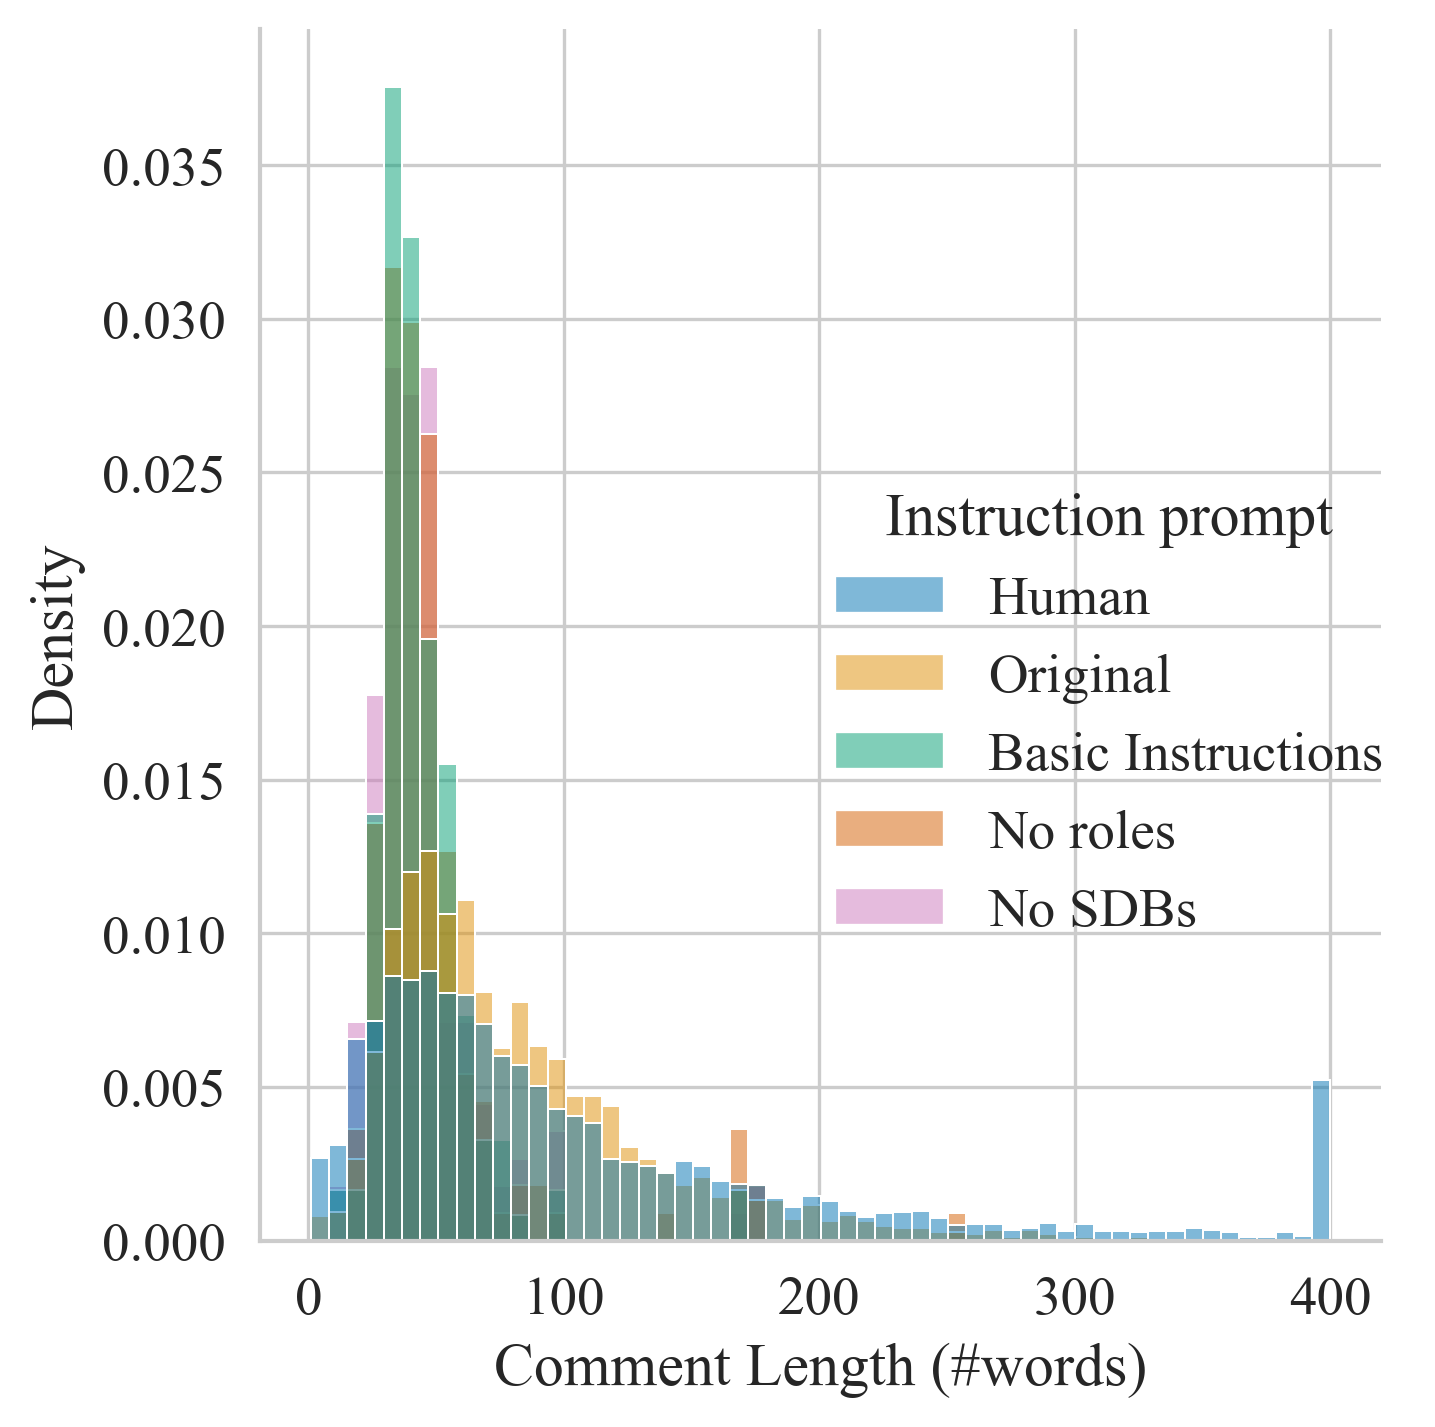
\includegraphics[width=0.32\linewidth]{comment_len_prompts.png}
	\centering
	\caption{Comment length for each discussion by model (Section~\ref{ssec:experimental:model}), turn-taking function $u$ (Section~\ref{ssec:experimental:turn}), and prompting function $\phi$ used (Section~\ref{ssec:experimental:prompts}). For ease of comparison, comments above $400$ words are marked at the end of the x-axis.}
	\label{fig::comment_length}
\end{figure*}

\begin{figure}[t]
    \centering
    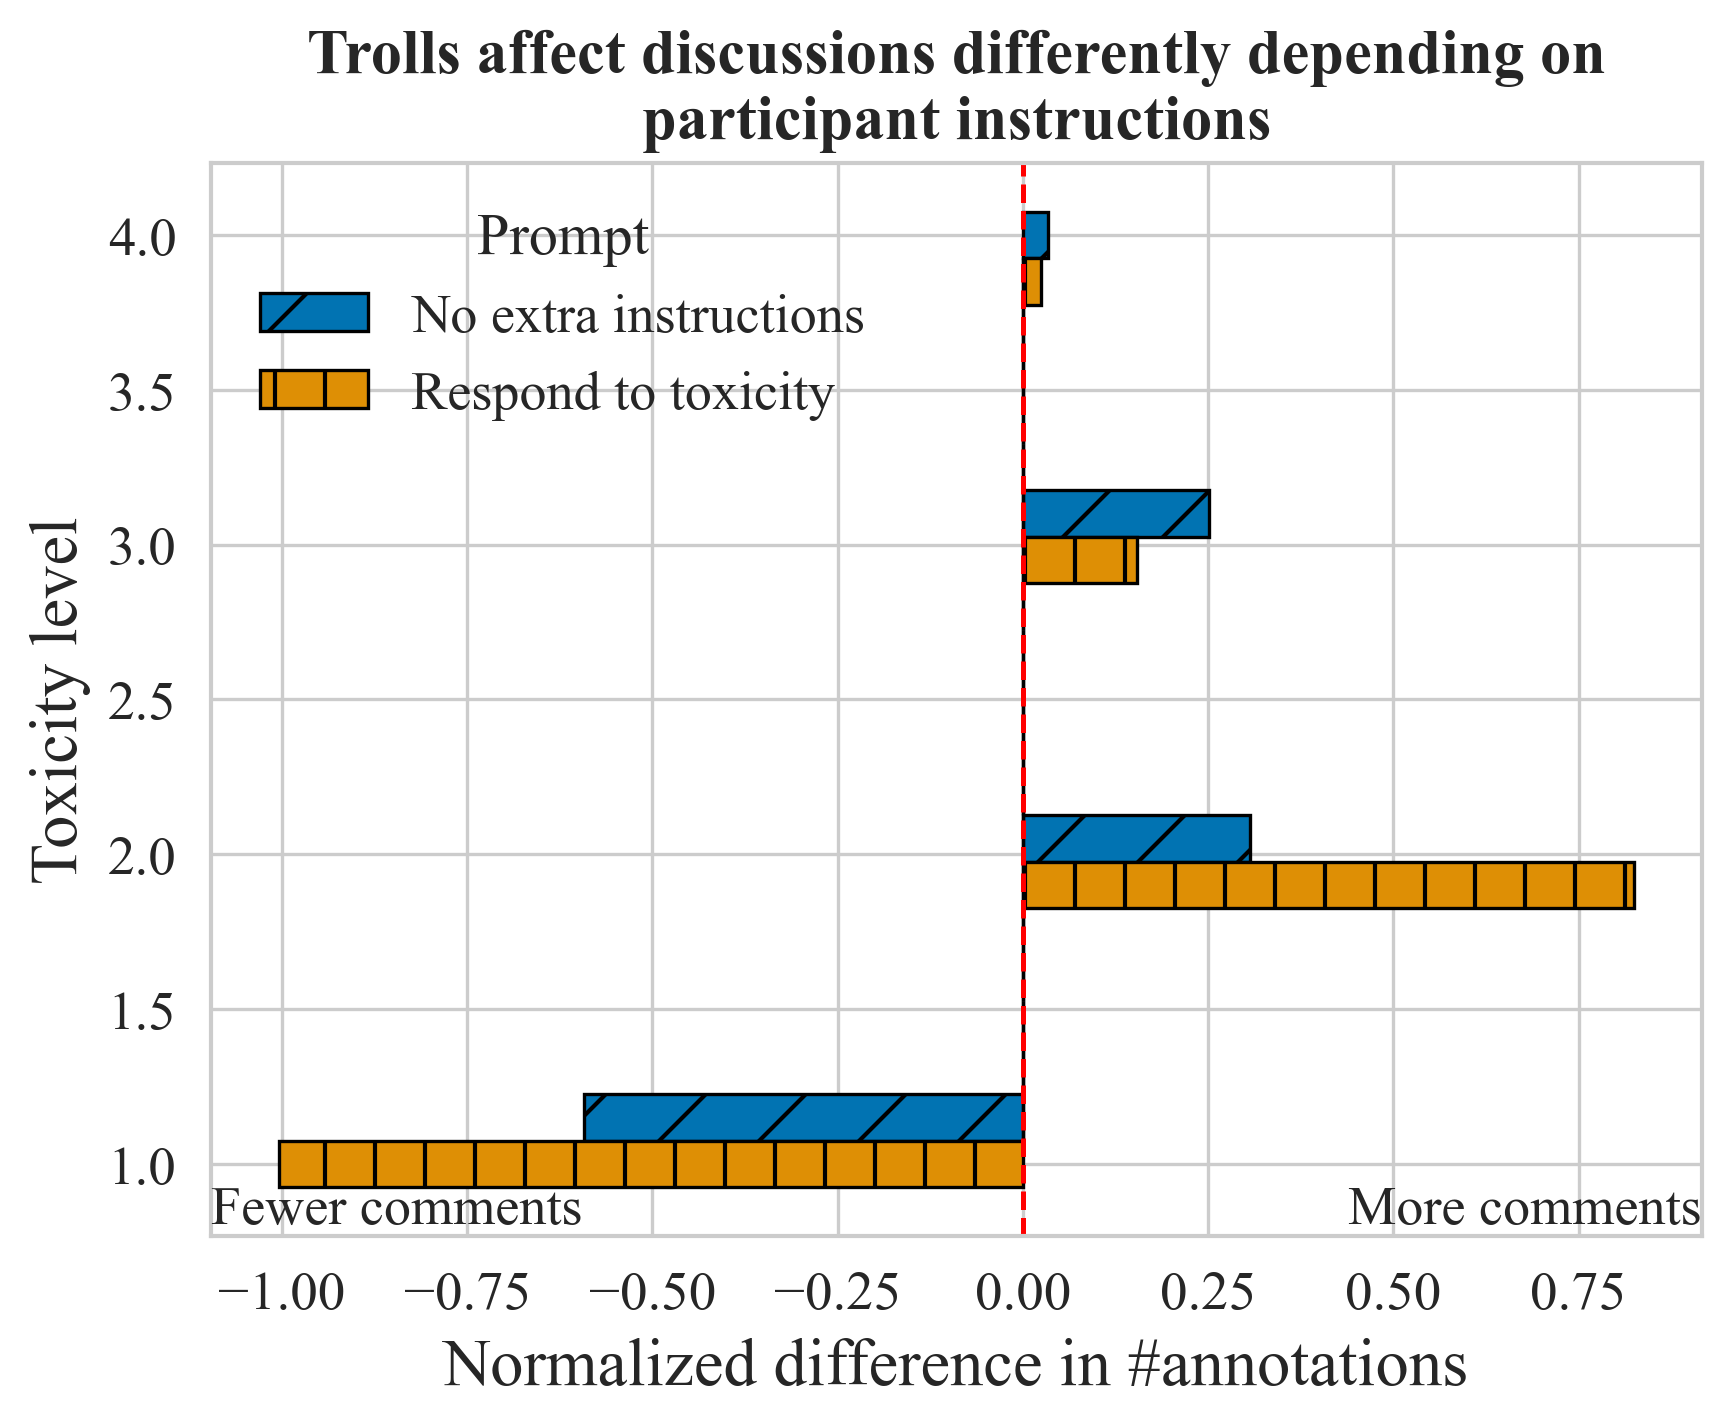
\includegraphics[width=0.49\linewidth]{toxicity_trolls.png} \hfill
    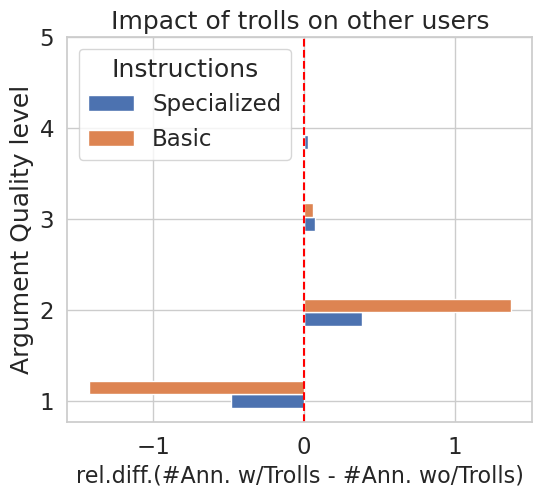
\includegraphics[width=0.49\linewidth]{aq_trolls.png}
    \caption{Relative differences in number of annotations by Toxicity (left) and \ac{AQ} (right) of synthetic discussions, excluding comments by troll user-agents. Comparison between our original (bottom, blue bars) and a basic instruction prompt (top, orange bars).}
    \label{fig::boxplots}
\end{figure}

